\documentclass{article}
\usepackage{graphicx} % Required for inserting images
\usepackage{hyperref}

\title{Hopper User Manual}
\author{Team 1000 - SENG302}
\date{As of Sprint 5}

\begin{document}

    \maketitle

    \tableofcontents

    \section{Introduction}

    The production instance of Hopper can be found on \url{https://csse-s302g10.canterbury.ac.nz/prod/}. This is the website we will reference in this user manual. However, a staging instance also exists at \url{https://csse-s302g10.canterbury.ac.nz/test/}, and local instances can be created by cloning the Team 1000 repository from the University of Canterbury's EngGitlab here: \url{https://eng-git.canterbury.ac.nz/seng302-2023/team-1000/}, and running the command \texttt{./gradlew bootRun}.

    \section{Accounts}

    \subsection{Registering an Account}

    In order to access much of our website, you must first register an account.

    You can access the registration page by clicking the register button in the top right, or by manually navigating to \texttt{/register}. Fill out the registration form your name (first and last are both required -- sorry Vincent), email address, date of birth, and a password. All users must be at least 13 years old to use Hopper.

    Your password must also meet certain metrics for strength. Your password must contain at least 8 characters, at least one upper case letter, at least one lower case letter, at least one number, and at least one other `special' character. You can see these metrics by hovering over the (?) icon. You must then retype this password exactly in the `Confirm Password' box to confirm that you have written it correctly.

    If any field has not been entered correctly, then clicking the `Register' button will display an error on the field that contained the error and a message explaining what the error was.

    \begin{figure}
        \centering
        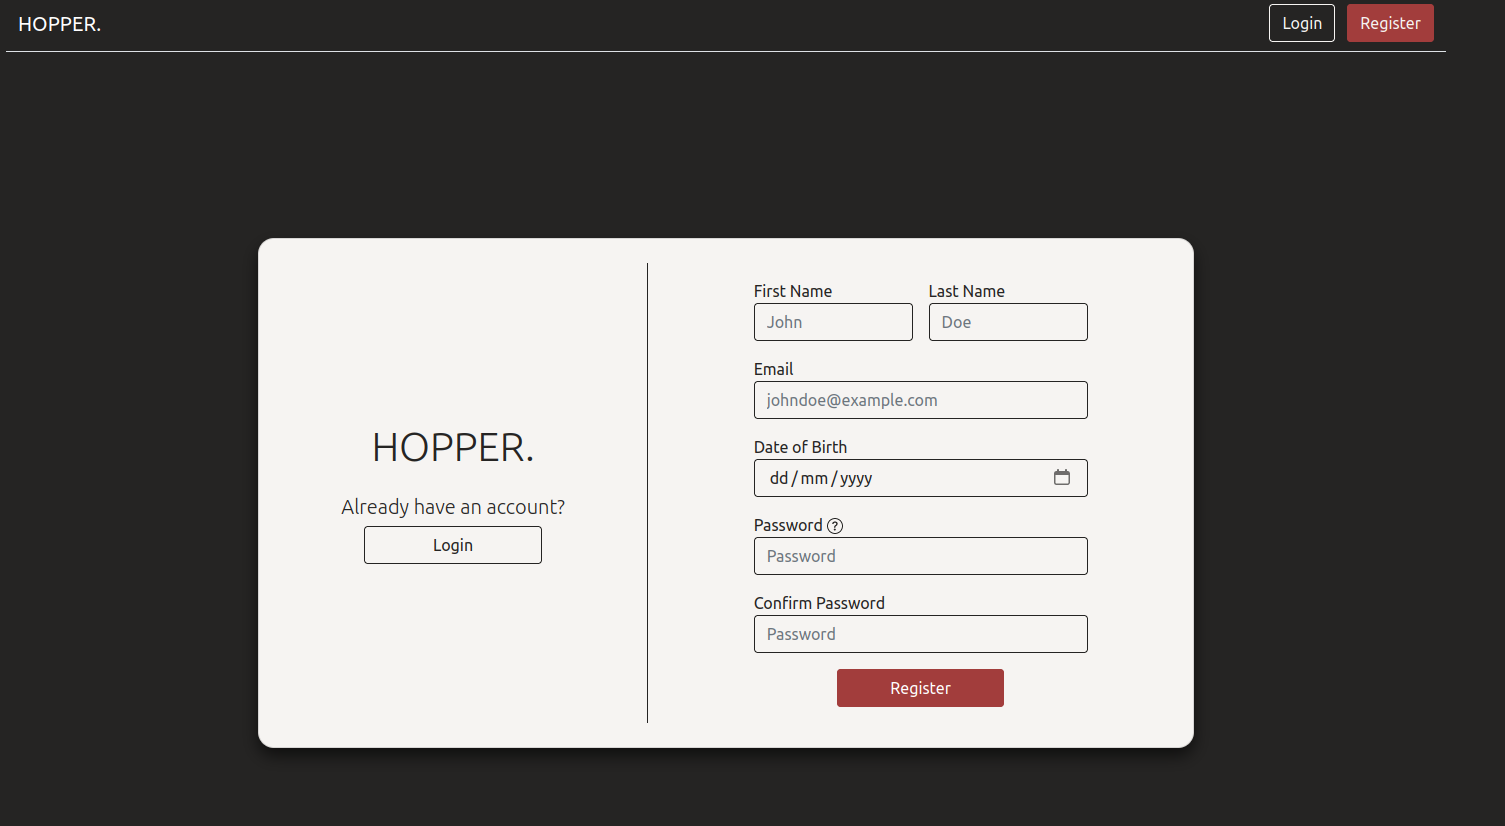
\includegraphics[width=\textwidth]{./register_page.png}
        \caption{The Hopper registration page}
        \label{fig:register}
    \end{figure}

    \subsection{Email Confirmation}

    Once you have finished entering your user information, press the `Register' button to register an account with Hopper. Assuming you have done so correctly, you will be brought to page asking you to confirm your email address. You will also be sent an email from the address \texttt{seng302team1000@gmail.com} will be sent to the email address that your provided in the registration form with a link to confirm your account. This email may also be sent to you randomly and without warning if your name is Miguel Morales. It may take a few minutes for this email to send, and it may end up in the junk folder. Clicking the provided link will then bring you to the login page and show a message confirming your account has been activated and then you must log in using the credentials you provided during the registration process to begin using Hopper.

    If you attempt to log in to your account before confirming your email address, then you will not be able to do so and an error message showing that your account still needs to be activated will be shown.

    You must confirm your email address within 2 hours of creating your account, otherwise it will be automatically deleted and you will have to register a new account again.

    \begin{figure}
        \centering
        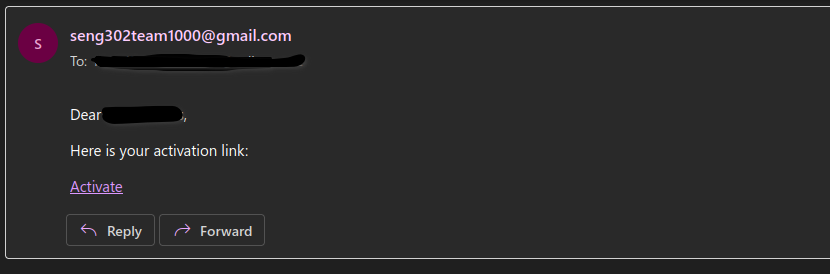
\includegraphics[width=\textwidth]{./confirm_email_address.png}
        \caption{The `confirm your email address' email, as seen in the Outlook web client. The recipient's name and email address have been intentionally redacted.}
        \label{fig:confirm_email}
    \end{figure}

    \subsection{Login and Password Resets}

    Once you have created an account for Hopper and confirmed your email address, you can login. You can do this by simply entering your email address and password, and then you will be directed to the home page.

    \begin{figure}
        \centering
        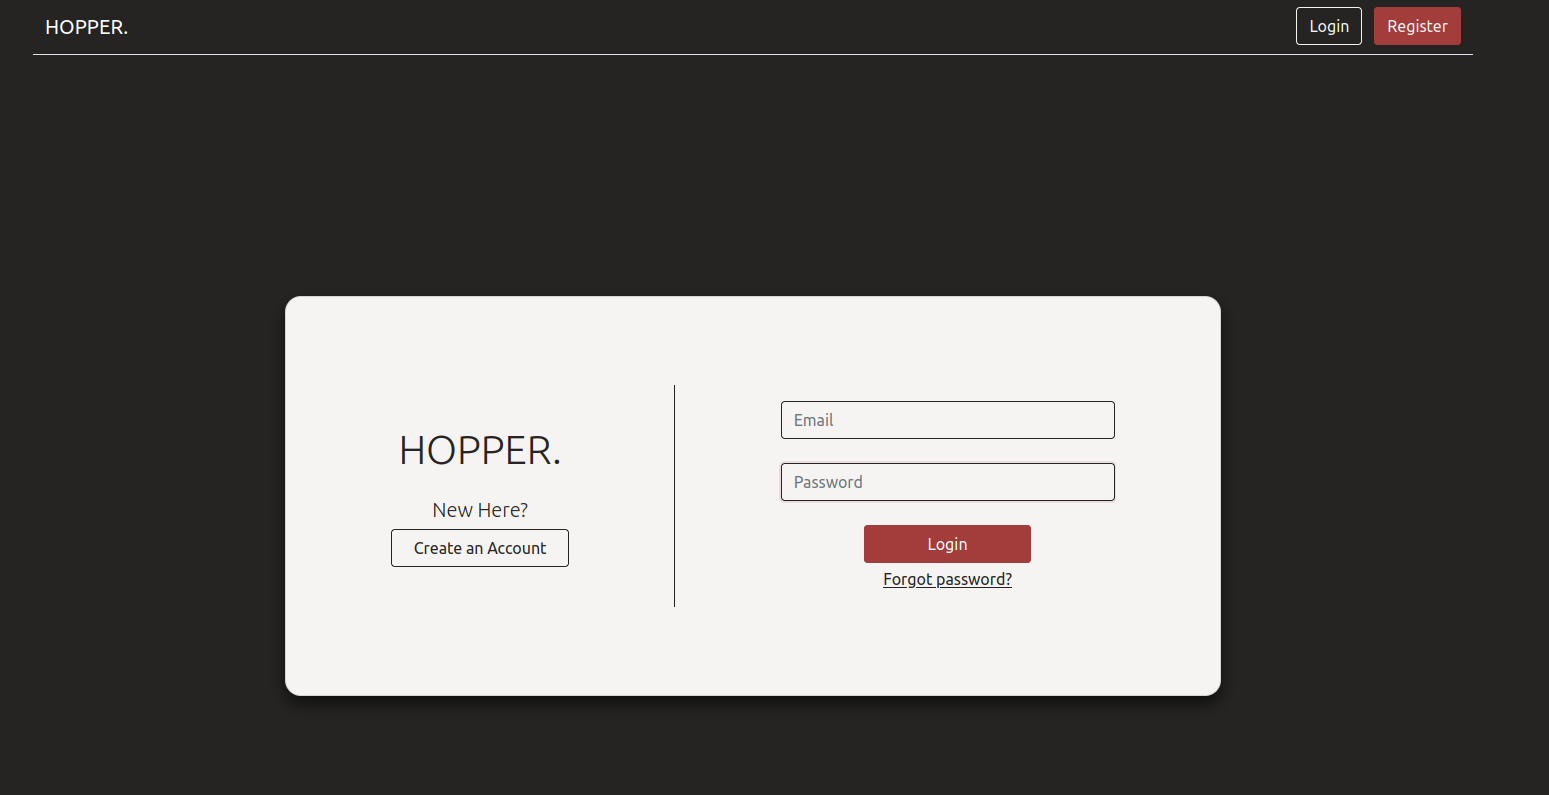
\includegraphics[width=\textwidth]{./login_page.png}
        \caption{The Hopper login page}
        \label{fig:login}
    \end{figure}

    If you forget your password, click the ``Forgot Password?" to begin the password reset process. Enter your user's email address into the text box provided, and a password reset link will be sent to that email address from the address \texttt{seng302team1000@gmail.com}. If you enter some other email address, the success message will still be displayed, though an email may or may not be sent. So, make sure you entered the correct email!

    Once you click the link, you will be taken to the reset password form. Enter a new password into the `New Password' field and then retype the password exactly in the `Retype Password` field. The new password must match the exact same strength requirements from the Registration page. If you enter something incorrectly, or your new password does not meet the same strength requirements, then an error will be displayed on the field with an error message telling you what you did wrong.

    Once you enter a valid new password and retype it correctly, clicking the `Reset Password' button will then reset your password and direct you to the login page. For security reasons, you must login again using the new password.

    \begin{figure}
        \centering
        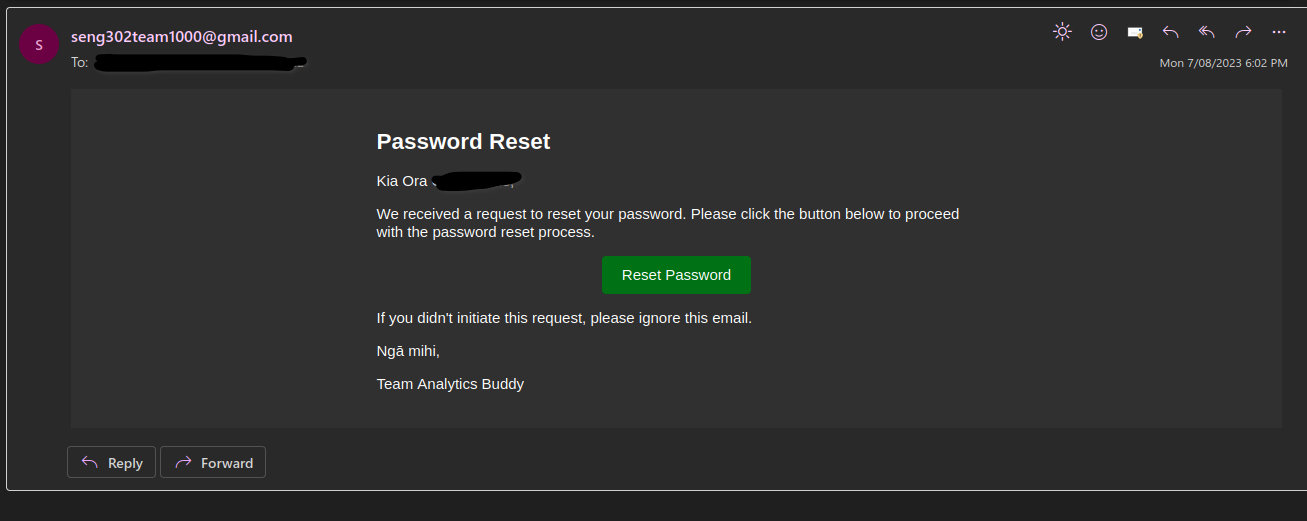
\includegraphics[width=\textwidth]{./password_reset_email.png}
        \caption{The `reset your password' email, as seen in the Outlook web client. The recipient's name and email address have been intentionally redacted.}
        \label{fig:password_reset}
    \end{figure}

\end{document}
